% tQRTguide.tex
% v1.2 released August 2014

\documentclass{tQRT2e}
\usepackage{fontspec}
\usepackage{subfigure}% Support for small, `sub' figures and tables
\usepackage{multirow}
\begin{document}

%\jvol{00} \jnum{00} \jyear{2014} \jmonth{August}

% \articletype{GUIDE}% NOT NEEDED FOR A RESEARCH ARTICLE IN THIS JOURNAL%

\title{Detection of Insulation Flaws and Thermal Bridges in Insulated Truck Box Panels}

\author{Lei, Lei$^{\rm a}$$^{\ast}$\thanks{$^\ast$Corresponding author. Email: lei.lei.1@ulaval.ca
\vspace{6pt}},  Alessandro Bortolin$^{\rm b}$, Paolo Bison$^{\rm b}$ and Xavier Maldague$^{\rm a}$\\\vspace{6pt}  $^{a}${\em{Computer Vision and Systems Laboratory, University Laval, Quebec, Canada}};
$^{b}${\em{CNR-ITC Padova, Italy}} \\\received{} }

\maketitle

\begin{abstract}
This paper focuses on the detection of defects and thermal bridges in insulated truck box panels, utilizing Infrared thermography. Unlike the traditional way in which passive thermography is applied, this research uses both heating and cooling methods in active thermography configurations. Lamp heating is used as the hot external stimulation, while a compressed air jet is applied as the cold external stimulation. An IR camera captures the whole process. In addition, numerical simulations under COMSOL$^®$ platform are also conducted. Experimental and simulation results for two situations are compared and discussed.

\begin{keywords}IR Thermography; Liquid Nitrogen Cooling;
COMSOL; Truck panel; Thermal Bridge
\end{keywords}

% \centerline{\bfseries Index to information contained in this guide}\vspace{12pt}

% \hbox to \textwidth{\hsize\textwidth\vbox{\hsize18pc
% \hspace*{-12pt} {1.}    Introduction\\
% \hspace*{7pt} {1.1.}  The {\it tQRT} document class\\
% \hspace*{7pt} {1.2.}  Submission of \LaTeX\ articles\\
% \hspace*{24pt}        to the journal\\
% {2.}    Using the {\it tQRT} class file\\
% {3.}    Additional features\\
% \hspace*{10pt}{3.1.}  Footnotes to article titles\\
% \hspace*{24pt}        and authors' names\\
% \hspace*{10pt}{3.2.}  Abstracts\\
% \hspace*{10pt}{3.3.}  Lists\\
% \hspace*{10pt}{3.4.}  Landscape pages\\
% {4.}    Some guidelines for using\\
% \hspace*{6pt}        standard features\\
% \hspace*{10pt}{4.1.}   Sections\\
% \hspace*{10pt}{4.2.}   Illustrations (figures)\\
% \hspace*{10pt}{4.3.}   Tables\\
% \hspace*{10pt}{4.4.}   Theorem-like environments\\
% \noindent \hspace*{7pt} {4.5.}   Typesetting mathematics\\
% \hspace*{24pt} {4.5.1.}   Displayed mathematics\\
% \hspace*{24pt} {4.5.2.}  Bold math italic symbols\\
% \hspace*{24pt} {4.5.3.}   Bold Greek\\
% \hspace*{24pt} {4.5.4.}   Upright Greek characters  \\
% \hspace*{50pt}             and the upright partial \\
% \hspace*{50pt}             derivative sign  \\}
% \hspace{-24pt}\vbox{\noindent\hsize18pc
% \hspace*{7pt} {4.6.}   Acknowledgements \\
% \hspace*{7pt} {4.7.}   Funding \\
% \hspace*{7pt} {4.8.}   Notes \\
% \hspace*{7pt} {4.9.}   Supplemental material \\
% \hspace*{7pt} {4.10.}   References \\
% \hspace*{24pt} {4.10.1.}   References cited in the\\
% \hspace*{54pt}             text  \\
% \hspace*{24pt} {4.10.2.}   The list of references\\
% \hspace*{7pt} {4.11.}   Appendices \\
% \hspace*{7pt} {4.12.}   {\it tQRT} macros  \\
% {5.}    Example of a section heading \\*
% \hspace*{6pt}   including {\fontencoding{T1}\scshape{small caps}}, {\it italic}, \\
% \hspace*{6pt}   and bold Greek such as ${\bm\kappa}$ \\
% {6.}   {\em tQRT} journal style \\
% \hspace*{10pt}{6.1.}   Hyphens, en rules, em rules \\ \hspace*{27pt}and minus signs\\
% \hspace*{10pt}{6.2.}   References \\
% \hspace*{10pt}{6.3.}   Maths fonts\\
% {7.}   Troubleshooting\\
% {8.}   Fixes for coding problems\\
% {9.}   Obtaining the tQRT2e class file\\
% \hspace*{10pt}{9.1}  Via the Taylor \& Francis website\\
% \hspace*{10pt}{9.2}   Via e-mail\\
%       }}
\end{abstract}


\section{Introduction}

% In order to assist authors in the process of preparing a manuscript for the {\itshape Quantitative InfraRed Thermography Journal} ({\it tQRT}), the journal's layout style has been implemented as a \LaTeXe\ class file based on the {\tt article} document class. A \textsc{Bib}\TeX\ style file is also provided to assist with the formatting of your references in a style appropriate to that of the journal.

% Commands that differ from or are provided in addition to the standard \LaTeXe\ interface are explained in this guide. The guide alone is not intended as a substitute for an appropriate \LaTeXe\ manual.

% The {\tt tQRTguide}.tex file can also be used as a template for composing an article for submission by cutting, pasting, inserting and
% deleting text as appropriate, using the \LaTeX\ environments provided (e.g. \verb"\begin{equation}",
% \verb"\begin{enumerate}").

% {\bf{Please note that the index following the abstract in this guide is provided for information only. An index is not required in submitted papers.}}


% \subsection{The {\bi tQRT} document class}\label{S1.1}

% The \textit{tQRT} class file preserves the standard \LaTeXe\ interface such that any document that can
% be produced using \texttt{article.cls} can also be produced with minimal alteration using the \textit{tQRT} document class.
% However, the measure (the width of the text on a page) differs from the default for \texttt{article.cls}, therefore line breaks
% will change and some long equations may need to be reformatted accordingly.

% If your article is accepted for publication in the journal, it will be typeset in Monotype Times. As most authors do not own this font, it is likely that the page make-up will alter slightly with the change of font. Please therefore ignore details such as slightly long lines of text, page stretching, figures or tables not being in exact synchronization with their citations in the text: these details will be dealt with by the typesetter. Similarly, it is unnecessary to spend time addressing warnings in the log file -- if your .tex file compiles to produce a PDF file that correctly reflects how you wish your paper to appear, such warnings will not prevent your source files being imported into the typesetter's program.


% \subsection{Submission of \LaTeX\ articles to the journal}\label{S1.2}

% Manuscripts for possible publication in the journal should be submitted to the Editors for review as directed in the journal's Instructions for Authors, which may be found at {\tt{http://www.tandf.co.uk/journals/authors/tqrtauth.asp}}.

% Manuscripts created using \LaTeX\ should be converted to PDF format prior to submission. The \LaTeX\ source files and any graphics files will be required in addition to the final PDF version when final, revised versions of accepted manuscripts are submitted.

% `Open-source' \LaTeXe\ should be used in preference to proprietary systems such as TCILaTeX or Scientific WorkPlace; similarly, class files such as REVTeX 4.1 that produce a document in the style of a different publisher and journal should not be used for preference.

% Authors who wish to incorporate Encapsulated PostScript artwork directly in their articles can do so by using
% Tomas Rokicki's {\tt EPSF} macros (which are supplied with the DVIPS PostScript driver). See Section~\ref{eps},
% which also demonstrates how to treat landscape pages. Please remember to supply any additional figure macros you
% use with your article in the preamble before \verb"\begin{document}". Authors should not attempt to use
% implementation-specific \verb"\special"s directly.

% Ensure that any author-defined macros are gathered together in the source file, just before the
% \verb"\begin{document}" command.

% Please note that if serious problems are encountered with the coding of a paper (missing author-defined macros,
% for example), it may prove necessary to divert the paper to conventional typesetting, i.e. it will be re-keyed.
The increasing cost of energy has made energy saving a vital necessity in the current world. One of the examples involves, “Maintaining the cold chain”: the correct transport of perishable foodstuffs in refrigerated vehicles, especially for dairy products, meat and frozen foods, which has become the key part of every successful distributor’s food safety program. Therefore, a suitable thermal insulation implemented in refrigerated vehicles is essential for saving energy while maintaining an appropriate conservation of the foodstuffs. There are some agreements concerning thermal insulation tests which ensures the suitability for the transport of food in refrigerated conditions, for example ATP: “The Agreement on the Transport of Perishable foodstuffs” \cite{Geneva1970}, which establishes standards for the international transport of perishable food between the states that ratify the treaty since 1970.

The Construction Technologies Institute of the Italian National Research Council (ITC- CNR), our collaborator, hosts a wide testing facility for refrigerated vehicles or insulated roll containers and it is also authorized by the Italian Ministry of Transport to perform such ATP tests \cite{Tassou2009,dragano2009experimental}. The ATP standard test is a procedure that measures the insulating performance of truck panels with a global approach; however, if there are some local flaws or thermal bridges inside the panels, which could not be measured by ATP tests, then the insulation and the stability of the temperature can no longer be guaranteed. Usually truck panels are manufactured from composite insulated materials in order to ensure that the interior of the truck is maintained at a cold temperature \cite{Bortolin2015}. Therefore, this research attempts to detect the local flaws inside a truck panel specimen with a straightforward visualization.


\section{Samples \& Methods}

% If the file {\tt tQRT2e.cls} is not already in the appropriate system directory for \LaTeXe\ files, either
% arrange for it to be put there, or copy it to your working folder. In order to use the {\it tQRT} document class, replace the command
% \verb"\documentclass{article}" at the beginning of your document with the command \verb"\documentclass{tQRT2e}".

% The following document-class options should \emph{not} be used with the {\it tQRT} class file:
% %
% \begin{itemize}
%   \item {\tt 10pt}, {\tt 11pt}, {\tt 12pt} -- unavailable;
%   \item {\tt oneside}, {\tt twoside} -- not necessary, oneside is the default;
%   \item {\tt leqno}, {\tt titlepage} -- should not be used;
%   \item {\tt onecolumn} -- not necessary as it is the default style.
% \end{itemize}
% %
% The \texttt{geometry} package and commands associated with it should also not be used to adjust the page dimensions.
\begin{figure}
	%\begin{center}
	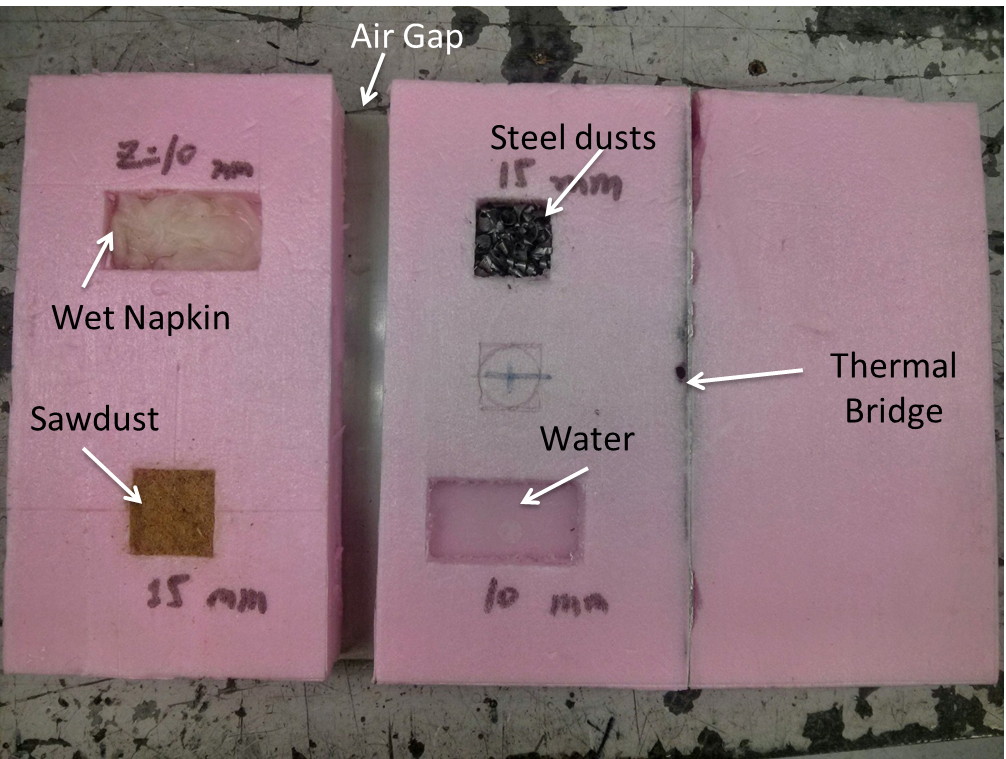
\includegraphics[width=7.33cm, height=5.5cm]{Panel_detail}
	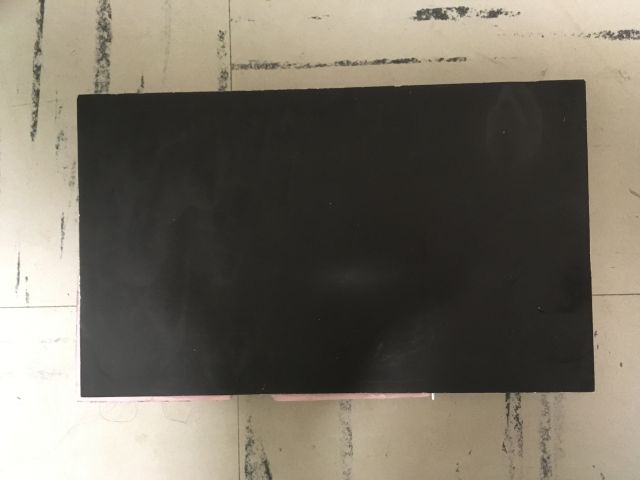
\includegraphics[width=7.33cm, height=5.5cm]{Panel_done}
	\caption{Details of defects inside the specimen (left) and final specimen to test (right) }
	\label{panel}
	%\end{center}
\end{figure}
\indent \indent In this research, several possible different types of defects inside a truck panel will be examined.  A panel containing these defects has been constructed and is shown in Figure~\ref{panel}. The insulated material used is Polystyrene, inserted between two thin Aluminum plaques. A small Aluminum plaque is embedded ‘vertically’ inside acting as a thermal bridge. Other flaws are defined as an air gap, a defect involving a wet napkin, a hole filled with sawdust, another hole filled with steel dust and a defect filled with water; these are representative of current truck box fabrication and potential defects. The simulated panel was painted before the test to increase emissivity of aluminum. Particularly the thermal bridge and the defect of water are the main targets to identify, since they appear regularly in the gaps of truck panels. A sound area with no defects has also been defined for later comparison and reference, which is located at the center of the specimen. The specification details can be found in Table~\ref{Tab_spe}:
\begin{table}
	\centering

	\caption{Specimen specification details.}
	\begin{tabular}{c|c|c|c|c}
		\hline
		& \textbf{Aluminum,plaques} & \textbf{Foam}       & \textbf{Air Gap}     & \textbf{Thermal Bridge} \\ \cline{2-5} 
		\multirow{2}{*}{Dimensions (mm)} & 250*150*1        & 250*150*25 & 15*150 *25  & 1*150*25       \\ \cline{2-5} 
		& \textbf{Wet Napkin}       & \textbf{Sawdust}    & \textbf{Steel dusts} & \textbf{Water}          \\ \cline{2-5} 
		& 40*20*10         & 20*20*15   & 20*20*15    & 40*20*10       \\ \hline
	\end{tabular}
	\label{Tab_spe}
\end{table}
%\begin{table}
%	\centering
%\tbl{Specimen specification details.}
%\begin{tabular}{lcccc}
%	\toprule
%	\multirow{4}{*}{\centering Dimensions (mm)}&
%	 Aluminum plaques & Foam & Air Gap & Thermal Bridge \\ 
%	 250*150*1 & 250*150*25 & 15*150*25 & 1*150*25 \\ 
%	 Wet Napkin & Sawdust & Steel dusts & Water \\ 
%	40*20*10 & 20*20*15 & 20*20*15 & 40*20*10 \\ 
%	\botrule 
%\end{tabular}
%\label{Tab_spe}
%\end{table} 
% \begin{table}
% \tbl{Specimen specification details.}
% {\begin{tabular}[l]{@{}lcccccc}\toprule
%   Class$^{\rm a}$ & $\gamma _1$ & $\gamma _2$$^{\rm b}$
%          & $\langle \gamma \rangle$
%          & $G$ & $|{\bm f}|$ & $\theta _{c}$ \\
% \colrule
%   BL Lacs & 5 & 36 & 7 & $-4.0$ & $1.0\times 10^{-2}$ & 10$^\circ$ \\
%   FSRQs & 5 & 40 & 11 & $-2.3$ & $0.5\times 10^{-2}$ & 14$^\circ$ \\
% \botrule
% \end{tabular}}
% \tabnote{$^{\rm a}$This footnote shows what footnote symbols to use.}
% \tabnote{$^{\rm b}$This footnote shows the text turning over when a long footnote is added.}
% \label{sample-table}
% \end{table}
In order to localize the possible defects inside the specimen, active Infrared Thermography \cite{Maldague2001theory,Balageas2016}, one of the Non-destructive Testing \& Evaluation techniques, is applied for diagnostics. Basically, the specimen to inspect is thermally stimulated and the subsequent temperature evolution is recorded to reveal possible subsurface flaws. In this study two opposing approaches of external stimulations are then applied with the goal of clearly detecting the flaws in the truck panel. One approach uses a traditional lamp heating; the other method involves air cooling. 


% \section{Additional features}
\section{Experimental set-up}
The experiment is set up with the following equipment, shown in Figure~\ref{Exp}:
\begin{figure}
	\centering
	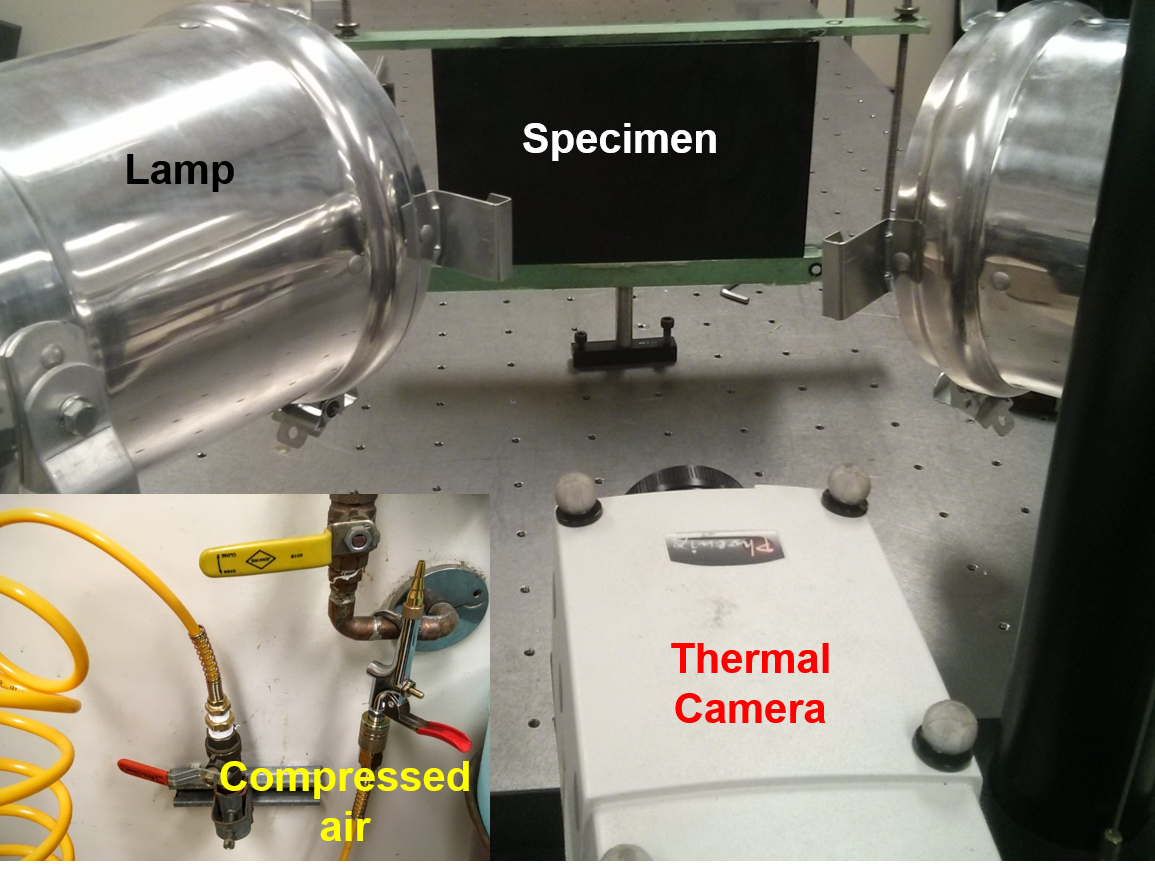
\includegraphics[scale=0.5]{Exp}
	\caption{Experimental Set-up}
	\label{Exp}
\end{figure}

\begin{itemize}
  \item Two halogen lamps each with heat source of 500W;
  \item A FLIR Phoenix thermal camera (640×512 pixels, InSb, 3-5 μm);
  \item Compressed air connected by a tube and a nozzle with a diameter of 5mm (Zoomed bottom left).
\end{itemize}

The whole procedure of study is described as follows:  

For lamp heating, two halogen lamps each with a total heat source of 1000$ W $ are employed at a distance of 0.4 $ m $ and at an angle of about 45° for the purpose of homogeneously heating the surface. The duration of the heating process is only 20 $ s $.   

For air-cooling, compressed air with a temperature of about 15° (details are shown in Table~\ref{air_cool}) is sprayed at a distance of 0.4$ m $ and at an angle of about 45° in the \textbf{left} front of the specimen’s surface. It is a central spray form left to right along the specimen surface. By doing this, one tries to avoid the direct squirt on the area of defects. In this process, contrary to the heating one, the specimen was preheated to about 30$ °C $, which is similar to the real situation for detection of truck panel defects in the summer. The duration of the cooling-down process is about 20 $ s $ as well.   
 \begin{table}
 \tbl{Air-Cooling parameters.}
 {\begin{tabular}[l]{@{}cccccc}\toprule
   \textbf{Material} & \textbf{Outlet Pressure} & \textbf{Flow}
          & \textbf{Nozzle diameter}
          & \textbf{Density} & \textbf{Temperature} \\
 \colrule
   Compressed Air & 6 bar & 0.0224 $m^3/s$ & 6.35 $mm$ & 1.2041 $kg/m^3$ & 15° \\
 \botrule
 \end{tabular}}
% \tabnote{$^{\rm a}$This footnote shows what footnote symbols to use.}
% \tabnote{$^{\rm b}$This footnote shows the text turning over when a long footnote is added.}
 \label{air_cool}
 \end{table}
Both processes have been recorded by the thermal infrared camera with a resolution of 640$\times$512 pixels.  

\section{Simulation models}
To obtain a comparative result, numerical models have also been developed, with the Finite Element Method under COMSOL Multiphysics$^{®}$. In addition to the similar transient problem appearing in experimental conditions, static regime simulation is also taken into account. The influences of heat conduction, convection and radiation (surface-to-surface and surface to ambient) on the heat flow through the defect have been simulated and analyzed.

The physical nature of the heat transfer is governed by the differential equations such as the one of the heat transfer by conduction, convection and radiation with temperature dependent thermal properties of materials involved. The differential equation, governing pure conductive heat transfer, to be solved on the model domain is: 

\begin{equation}
\rho C_p \frac{\partial T}{\partial t}-\nabla \cdot (k\nabla T) = 0
\end{equation}
where $\rho$ is the density (\textit{kg/m3}),   $C_p$ is the material heat capacity at constant pressure (\textit{J/(kg·K})), $ T $ is absolute temperature ($ K $) and \textit{k} is the material thermal conductivity (\textit{W/(m·K})) and $ t $ is the time.

The boundary condition included heat transfer by convection and radiation from the object surfaces and the  heat  source $q_0 $  applied on the front surface as the following: 
\begin{equation}
n(k\nabla T) = q_0 + h_{cv}(T_{amb}-T)+\sigma \epsilon(T_{amb}^4-T^4)
\label{eqf}
\end{equation}
where $ h_{cv} $ is the constant convective heat transfer coefficient, $\sigma$ is the Stefan-Boltzmann constant  and $\epsilon$ is the emissivity that is the ratio of radiant emittance of an object to that of a blackbody at the same temperature. Its value lies from zero for a non radiating object and 1.0 for a blackbody. $ T_{amb} $ is the Room temperature.
\begin{figure}
	%\begin{center}
	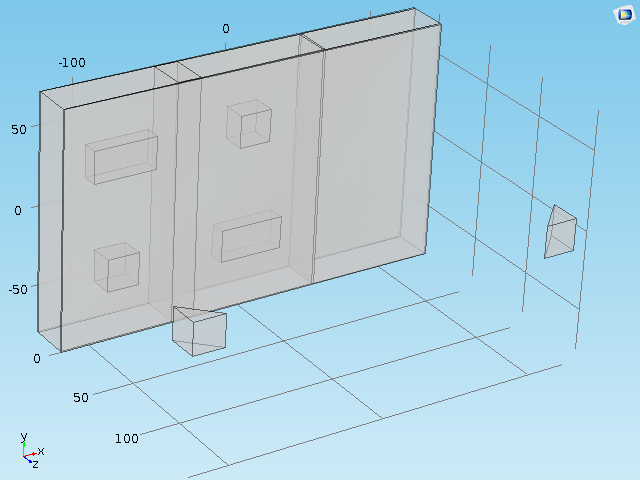
\includegraphics[width=7.33cm, height=5.5cm]{Flash_model2}
	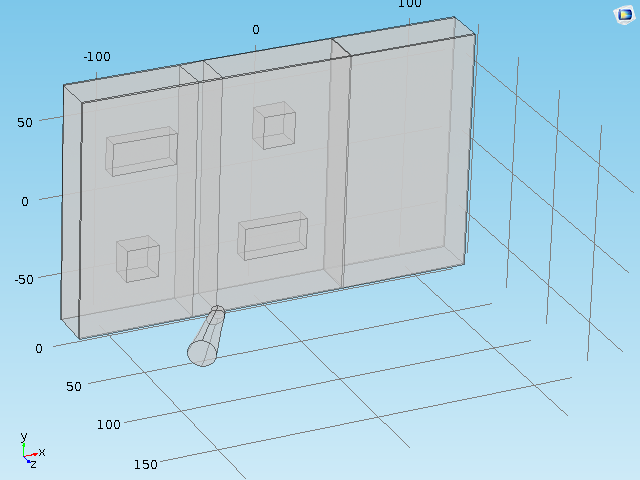
\includegraphics[width=7.33cm, height=5.5cm]{Laminar_model2}
	\caption{Simulation 3D models transparency view:  Heating with two halogen lamps (Left) and Cooling with compressed air by a nozzle (Right)}
	\label{models}
	%\end{center}
\end{figure}
Parameters for each model are introduced as follows:\\
For lamp heating, Heat Transfer in Solid with Surface-to-Surface Radiation module is applied in the model. Therefore, one assumes that there is no effect by convective transfer [$h_{cv}=0$ in eq. \ref{eqf}]

For air cooling, Heat transfer and Single Phase Laminar Flow modules are implemented since the convection effect in this case has a more significant influence. The Multiphysics setting is also set as a Non-Isothermal Flow. Then one assumes that there is no effect by the heat source [$ q_0=0 $ in eq. \ref{eqf}]

For the static regime, a simple Heat Transfer in Solid module is employed. Thus one has $ h_{cv} $=0 and $ q_0=0 $ in eq. \ref{eqf}

All materials properties applied in the models can be found in Table~\ref{mat_pro}. 
 \begin{table}[ht]
  	\centering
  	\scriptsize
 	\caption{Materials properties.}
% \tbl{Materials properties.}
 {\begin{tabular}{p{1.5cm}|p{1.5cm}p{1.5cm}p{1.5cm}p{1.5cm}p{1.5cm}p{1.5cm}}
 	\hline
	      & Density $\rho [Kg/m^3] $
	      & Thermal conductivity  $k [W/(m\cdot K)] $
          & Heat Capacity $C_p [J/(Kg\cdot K)]$
          & Surface Emissivity $\epsilon$
          & Dynamic viscosity $\mu [10^{-5}kg/m\cdot s]$ 
          & Ratio of specific heat $\gamma$   \\
	 \hline
   Aluminum (plaques and Thermal bridge)	&2700	&238	&900 &0.77 & & \\
   Foam	&24	&0.03	&1300 & & & \\
   Air	&1.2 &0.024	&1.005 & &1.846 &1.4 \\
   Sawdust	&192	&0.08	&900 & & & \\
   Water &1000	&0.58	&4.18 & & &1.33 \\
   Steel &7850	&44.5	&475 & & & \\
   Lamps &8700	&400	&10 &0.99 & & \\
	 \hline
 \end{tabular}}
% \tabnote{$^{\rm a}$This footnote shows what footnote symbols to use.}
% \tabnote{$^{\rm b}$This footnote shows the text turning over when a long footnote is added.}
 \label{mat_pro}
 \end{table}


\section{Results and Discussion}
Several image post-processing methods can be applied, such as Pulsed Phase Thermography \cite{Maldague1996}, Principal Component Thermography \cite{Rajic2002}. PCT technique uses “singular value decomposition (SVD) to reduce the matrix of observations to a highly compact statistical representation of the spatial and temporal variations relating to contrast information associated with underlying structural flaws”. Temperature distributions of the panel surface for both cases are presented in Figure~\ref{exp_res} and Figure~\ref{sim_res} (Front View). Both lamp-heating and air-cooling images shown are the third image post-processed by the PCT technique. It is clear that in experimental results, the defects of metal and water are easy to identify, in both heating and cooling cases. The Thermal bridges are slightly clearer in the cooling process than the heating process. However, the defect of the wet napkin has almost not been displayed in both cases. On the other hand, in simulation results, due to the ideal conditions, one can clearly notice the four defects mentioned above. Figure 5 indicates that there is a more obvious view of defects in lamp heating as opposed to air cooling, the detection time of the latter is much less.
\begin{figure}
%	\begin{center}
	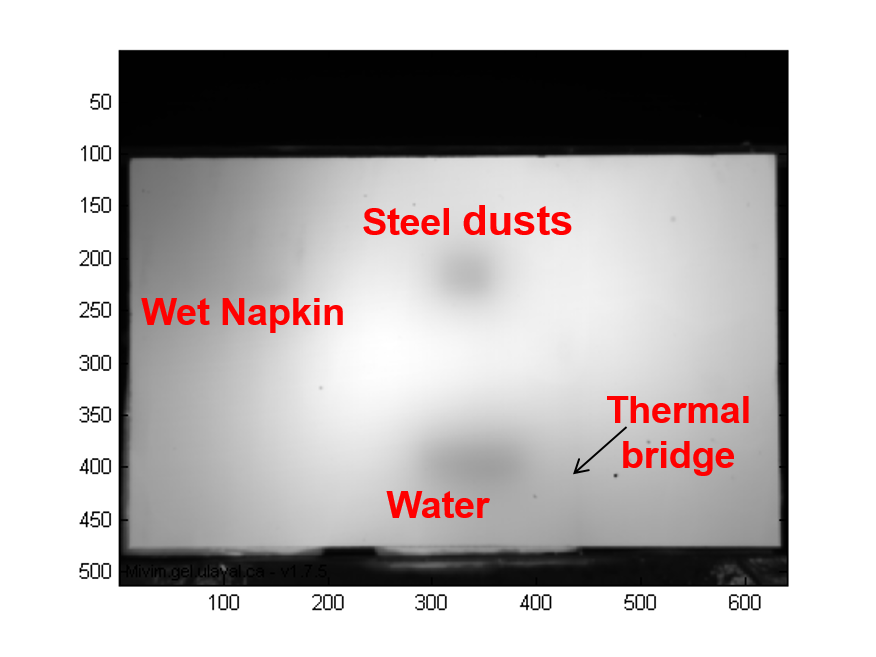
\includegraphics[width=7.8cm, height=5.85cm]{Heat_FT_AMP}
	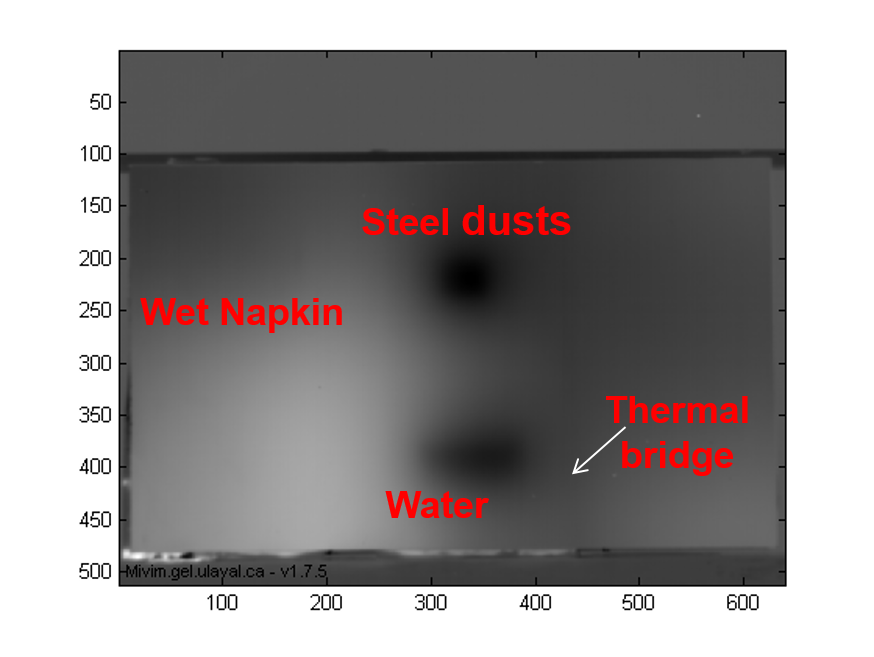
\includegraphics[width=7.8cm, height=5.85cm]{Cool_PCT3_2}
	\caption{Temperature distribution of panel surface with Lamp heating (left) and Air cooling (right) [Experiments]}
	\label{exp_res}
%	\end{center}
\end{figure}

\begin{figure}
%	\begin{center}
	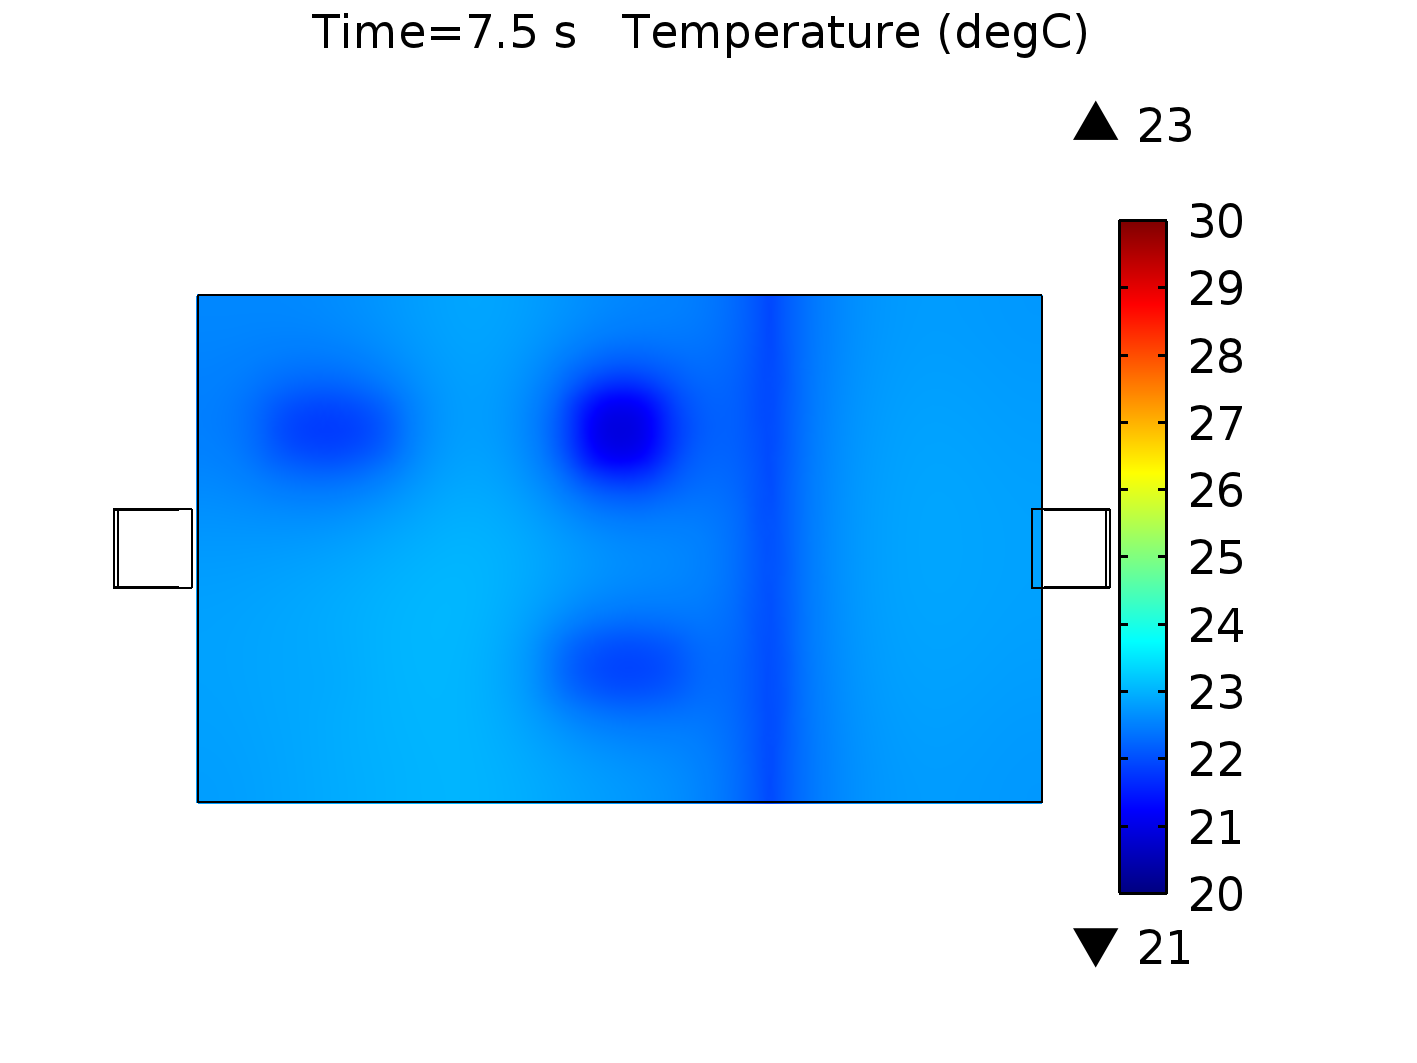
\includegraphics[width=7.8cm, height=5.85cm]{Truck_panel_flash_03}
	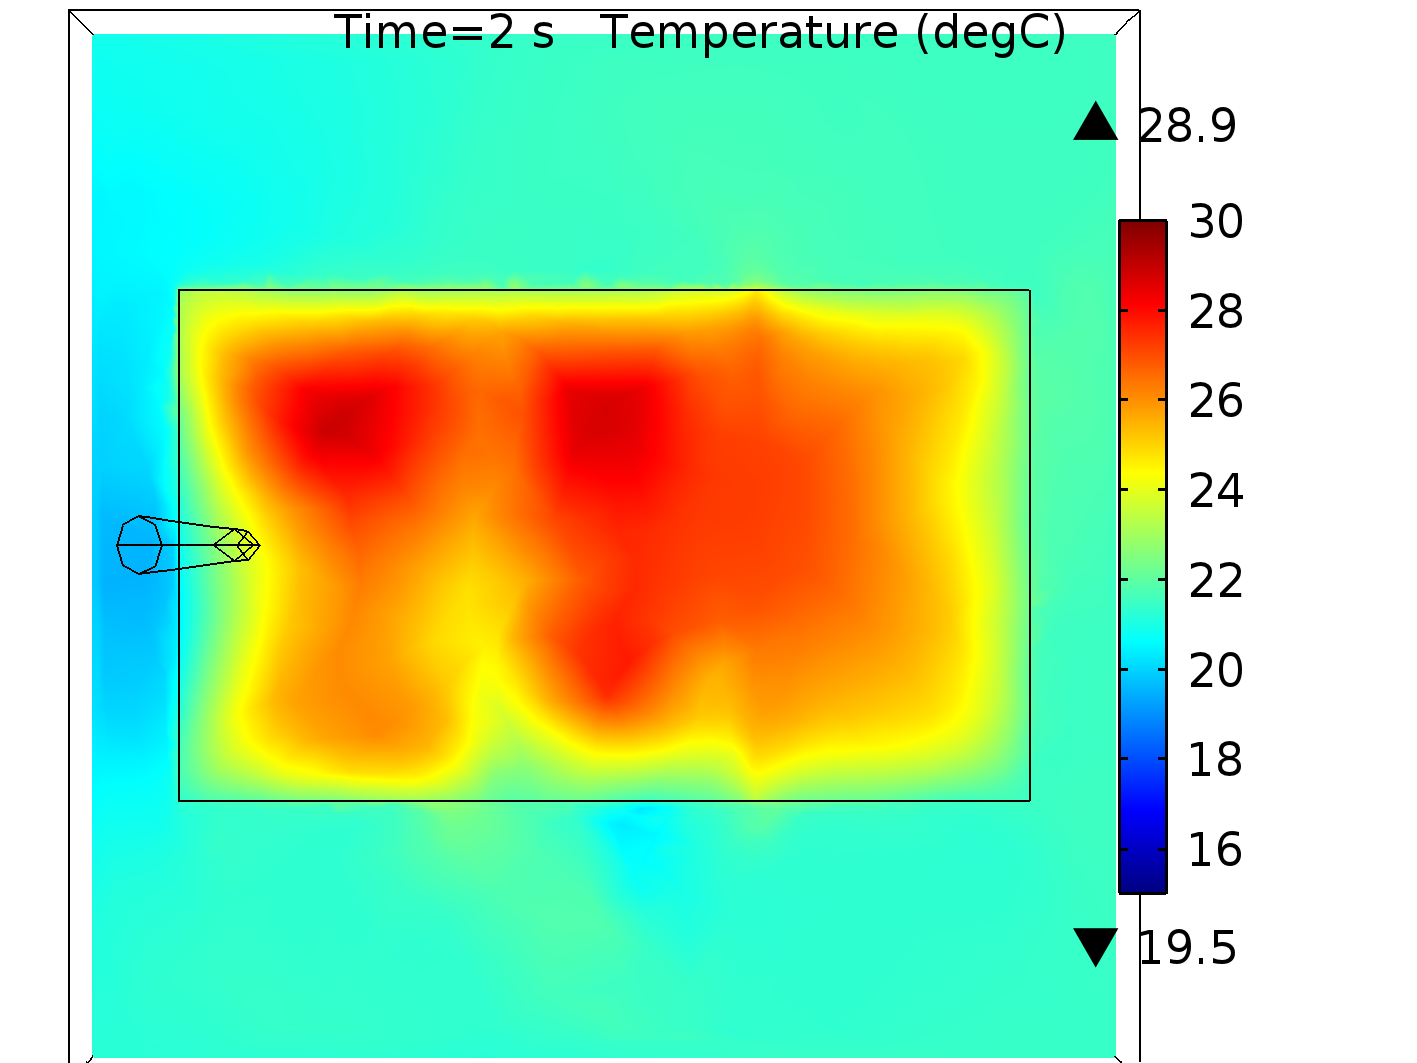
\includegraphics[width=7.8cm, height=5.85cm]{Truck_panel_laminar_final_7_3}
	\caption{Temperature distribution of panel surface with Lamp heating (left) and Air cooling (right) [Experiments]}
	\label{sim_res}
%	\end{center}
\end{figure}
Nonetheless, in both experiments and simulation models the sawdust defect was impossible to detect, due to its thermal conductivity close to Polystyrene. The same situation occurred for the air gap, which could not be detected, neither.  

From the observations above, a discussion of detectability of defects can be summarized as:
In comparison, both methods can only detect four defects rather than all. Although the halogen lamps were positioned to achieve a high energy pulse and a homogeneous heating as well, there is still an inhomogeneous distribution of temperature with a maximum in the middle of the sample and smaller values at the edges and especially in the area of wet napkin and sawdust (left edge part in the image). This might explain that wet napkin was displayed in computational results (ideal condition) while one could not detect it in real heating process. 

For air cooling, the jet impingement can not be neglected. Since the it was not an uniform spray to the sample surface, the squirt was produced in left center along the surface of the specimen to the right. Therefore, the areas of wet napkin and sawdust were not cooled well. The main part of air jet was deployed on the steel dust, water and thermal bridge defects zones. This might explain that in simulation model (ideal condition), at the first beginning of the cooling process the four defects appeared and in experimental test one could not observe the wet napkin defect.

In addition to the straight views comparison in the thermal images, the quantitative computation has also been carried out at the same time. Temperature evolutions in time for both cases are illustrated in Figure~\ref{exp_fig} and Figure~\ref{sim_fig}. Here one calculates the cases of the Water and Thermal Bridge (which are generally found in truck panels) compared to the Sound Area without defects. In both situations, experimental and simulation, it is observed that during lamp-heating, the temperatures of the thermal bridge and water defect area increased more slowly than the sound area value, while they decreased more slowly as well during air cooling. Quantitatively, for lamp heating, all defect temperature areas are lower than the sound area temperature. For air-cooling, on the contrary, all temperatures of defect areas are higher than that of the sound area (The descendant curve at the end of heating profile is due to the delay between the camera and lamps).  
\begin{figure}
	%	\begin{center}
	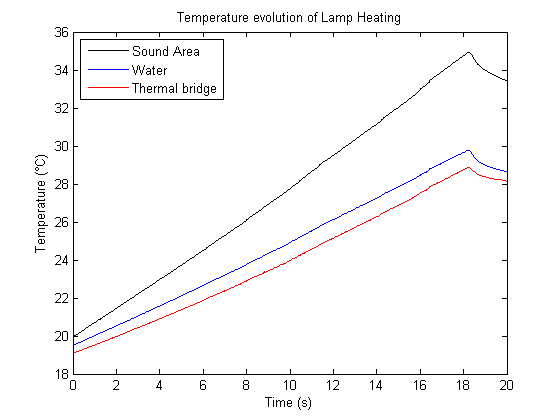
\includegraphics[width=8cm, height=6cm]{heating_evolution5}
	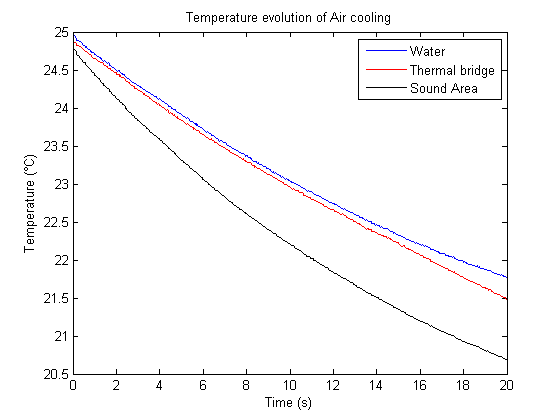
\includegraphics[width=8cm, height=6cm]{cooling_evolution4}
	\caption{Temperature distribution of panel surface with Lamp heating (left) and Air cooling (right) [Experiments]}
	\label{exp_fig}
	%	\end{center}
\end{figure}

\begin{figure}
	%	\begin{center}
	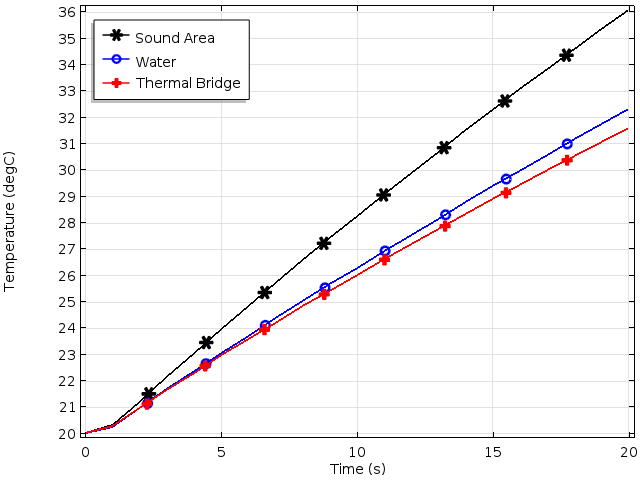
\includegraphics[width=8cm, height=6cm]{Truck_panel_Flash_TGraph_4}
	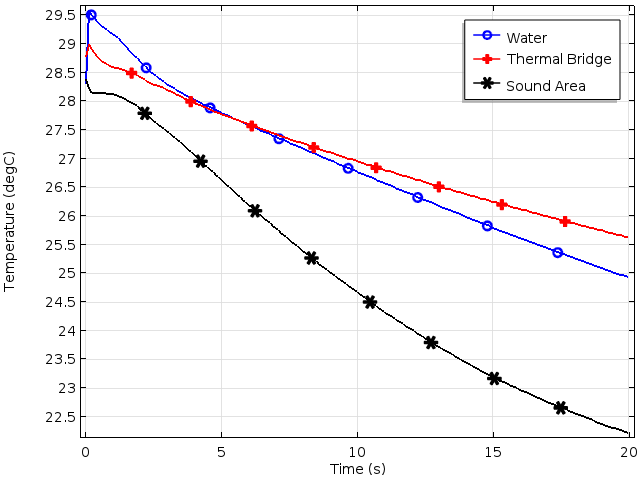
\includegraphics[width=8cm, height=6cm]{Truck_panel_laminar_TGraph_4}
	\caption{Temperature distribution of panel surface with Lamp heating (left) and Air cooling (right) [Experiments]}
	\label{sim_fig}
	%	\end{center}
\end{figure}
From the results above, one calculates the thermal contrasts between two defects and the sound area. Moreover, the corresponding contrast peaks have been determined, shown in Table~\ref{tab_TCP}:
\begin{table}[ht]
	\centering
	\caption{Thermal contrast peak table ($˚C$)}
	\begin{tabular}{l|cc|cc}
		\hline
		& \multicolumn{2}{c|}{Experiment} & \multicolumn{2}{c}{Simulation} \\
		 & Heating & Cooling & Heating & Cooling \\
		\hline
		Sound Area & 0 & 0 & 0 & 0 \\
		Water & 5.17 & 1.08 & 3.80 & 1.6 \\
		Thermal bridge & 6.07 & 0.87 & 4.52 & 2.3 \\
		\hline
	\end{tabular}
	\label{tab_TCP}
\end{table}
This table indicates that for both cases, the Lamp Heating method has a higher contrast peak than the Air Cooling method. While comparing the temperature evolution profiles, the Air Cooling method requires less time to reach the contrast peak. This coincides with the detection of flaws in thermal images view.

For further exploration of the detection of each method, one defines here a “Threshold” with Cp = 1 as the limit of detection, where Cp is the peak of thermal contrast. As the experimental and computational results are very comparable from above, we change the size (diameter) of the water defect and the thickness of thermal bridge in both heating and cooling models to seek the limit of detection. For supplementary comparison, we add also a regular situation: the static regime. This acts as the traditional passive thermography. One imagines that the truck is under sunshine in the exterior during summer, and inside temperature is kept as the cold chain, which should be -20°C. Then an infrared camera from outside observes the truck panel. Different sizes of water defects and widths of the thermal bridge have been performed during the same period (20$ s $) for this case.

All the computational results are presented in the following figures (Figure~\ref{sim_fig_stat} and Figure~\ref{sim_fig_ht})
\begin{figure}
	%	\begin{center}
	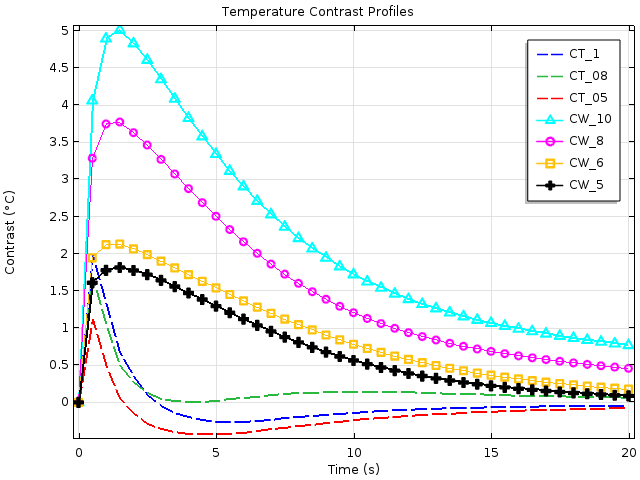
\includegraphics[width=8cm, height=6cm]{Truck_panel_Model_Static_Contrast}
	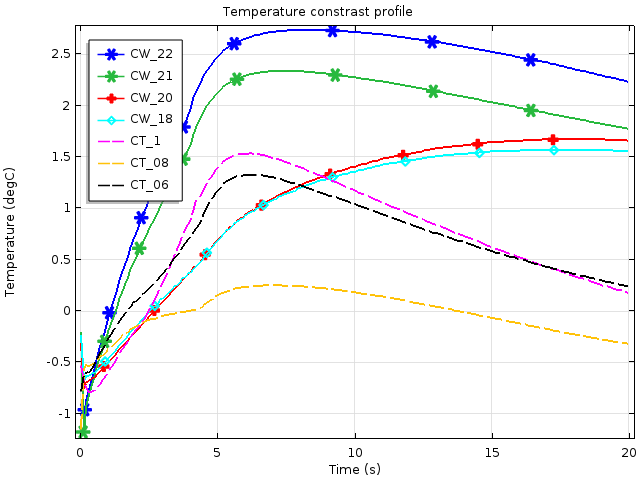
\includegraphics[width=8cm, height=6cm]{Truck_panel_Model_laminar}
	\caption{Temperature contrast profiles for models (Left: static regime; Right: Air cooling)}
	\label{sim_fig_stat}
	%	\end{center}
\end{figure}

\begin{figure}
	%	\begin{center}
	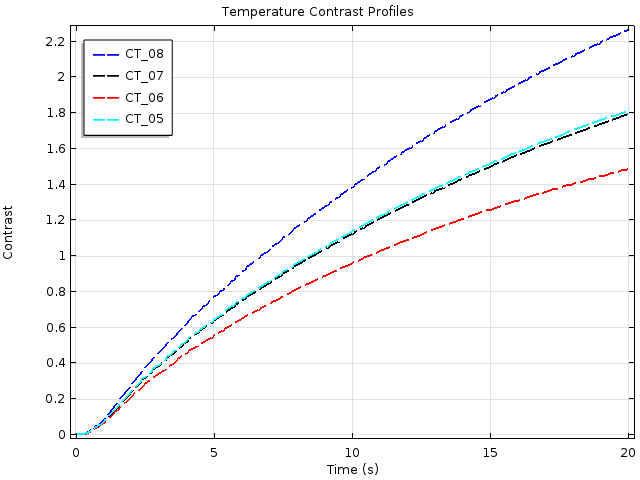
\includegraphics[width=8cm, height=6cm]{Truck_panel_Model_Flash_CT}
	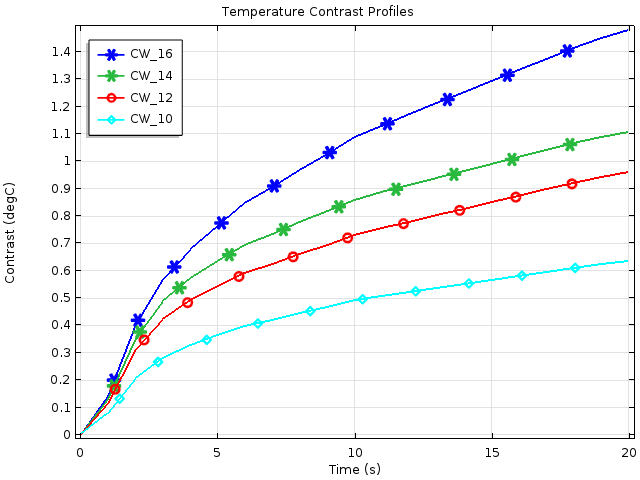
\includegraphics[width=8cm, height=6cm]{Truck_panel_Model_Flash_CW}
	\caption{Temperature contrast profiles for Lamp heating model (Left: thermal bridge, right: water defects)}
	\label{sim_fig_ht}
	%	\end{center}
\end{figure}
Where $ CT $ represents the contrast of the thermal bridge, $ CW $ represents the contrast of the water defect in all figures, and the numbers indicate the diameter and the thickness respectively. 

From the results above, it is evident that the static regime and lamp heating have more consistent profiles for the two types of flaws. All profiles in static regime increased rapidly at the beginning, as a consequence of temperature difference between sound area and defects area. Soon they all reached at a peak value subsequently. The contrast peak values varied according to different sizes of defect. Evidently, the contrast values of water defects are more sizable than that of thermal bridge. Then all profiles decreased gradually since the propagation of the heat inside the panel. In the end, they tend around whole uniform. 

While in air-cooling case there are several non-uniform profiles, nonetheless, the contrast profiles of water defect with large sizes (21 $mm $ and 22 $ mm $) and those of thermal bridge with all sizes have the similar tendency. They increased at the beginning due to the convection by air and then decreased slowly because of the propagation of heat dissipation inside the panel. However, for the contrast profiles of water defects with smaller sizes (20 $ mm $ and 18 $ mm $), they appeared as a unique increase. They might decrease again for long time modeling. An unusual thing found in air-cooling model was the thermal bridge with 0.8 $ mm $ thick had a lower contrast than those of 1 $mm $ and 0.6 $ mm $, this might be due to the influence of disturbance by airflow. 

For lamp-heating situation, one can observe that whole contrast profiles had a uniform tendency, which they all raised with time. This is as a result by radiation heating.

Finally, according to our “Threshold” $ C_p  = 1$, then from the figures the limit of detection of these three cases is (during a period of time [20$ s $]): 
\begin{itemize}
	\item Static regime: Water defect diameter 5 $ mm $; Thermal Bridge Thickness 0.5 $ mm $.
	\item Air cooing: Water defect diameter 18 $ mm $; Thermal Bridge Thickness 0.6 $ mm $.
	\item Lamp heating: Water defect diameter 14 $ mm $; Thermal Bridge Thickness 0.5 $ mm $.
\end{itemize}
One must note that, these results have been obtained by simulation models, which were undertaken in ideal situations. The results might be different in the real case.


\section{Conclusion}
This study concentrates on the detection of defects and thermal bridges in insulated truck box panels, by active Infrared thermography. Comparison between heating and cooling approaches for experiments and models has been established. In addition, passive thermography detection in computational models has been presented. Results demonstrate that the compressed air spray is more rapid than the traditional heating method in providing successful detection. Even if the traditional heating approach provides clearer results, in reality it is not easy and practical to heat a whole truck box to conduct inspection: the compressed air spray approach is much more convenient. 

A consideration of replacing compressed air by liquid nitrogen will be investigated in future work. What’s more, inspired from the static regime of simulation, a heat flux direction control may help improve the heat vertical propagation into the sample. Thus, deeper and smaller flaws inside the materials might be revealed more clearly. Based on these thoughts, a strategy of heating one side and cooling another side would be taken into consideration in future models and tests.


\section*{Acknowledgment}
This research was supported by the governments of Italy and Quebec, and by the Natural Sciences and Engineering Research Council of Canada (NSERC). We are also thankful to our collaborative institute CNR-ITC Padova which provided expertise that greatly helped in this research. 

\bibliographystyle{tQRT}
\bibliography{Biblio_th}


% \subsection{Footnotes to article titles and authors' names}

% On the title page, the \verb"\thanks" control sequence may be used to produce a footnote to either the title or authors' names. Footnote symbols for this purpose should be used in the order:
% $\dagger$ (coded as \verb"\dagger"), $\ddagger$ (\verb"\ddagger"), $\S$ (\verb"\S"), $\P$ (\verb"\P"), $\|$ (\verb"\|"), $\dagger\dagger$ (\verb"\dagger\dagger"),
% $\ddagger\ddagger$ (\verb"\ddagger\ddagger"),  $\S\S$ (\verb"\S\S"), $\P\P$ (\verb"\P\P"), $\|\|$ (\verb"\|\|").

% Any \verb"\footnote"s to the main text will automatically be assigned the superscript
%  symbols 1, 2, 3, etc. by the class file.\footnote{If preferred, the \texttt{endnotes} package
%  may be used to set the notes at the end of your text, before the bibliography.
%  The symbols will be changed to match the style of the journal if necessary by the typesetter.}

% The title, author(s) and affiliation(s) should be followed by the {\verb"\maketitle"} command. If preparing an anonymized version for peer review, {\verb"\maketitle"} may follow directly after the title in order to shield the authors' identities from the reviewers.


% \subsection{Abstracts}

% At the beginning of your article, the title should be generated in the usual way using the {\verb"\maketitle"}
% command. Immediately following the title you should include an abstract. The abstract should be enclosed within
% an {\tt abstract} environment. For example, the titles for this guide were produced by the following source code:
% %
% \begin{verbatim}
% \title{{\itshape Quantitative InfraRed Thermography Journal}\break
% \LaTeX\ style guide for authors (Style 2 + NLM reference style)}

% \author{A.N. Author$^{\rm a}$$^{\ast}$\thanks{$^\ast$Corresponding
% author. Email: latex.helpdesk@tandf.co.uk \vspace{6pt}} and I.T.
% Consultant$^{\rm b}$\\\vspace{6pt} $^{a}${\em{Taylor \& Francis,
% 4 Park Square, Milton Park, Abingdon, UK}}; $^{b}${\em{Institut
% f\"{u}r Informatik, Albert-Ludwigs-Universit\"{a}t, Freiburg,
% Germany}}\\\received{v1.2 released August 2014} }

% \maketitle

% \begin{abstract}
% This guide is for authors who are preparing papers for the Taylor \&
% Francis journal {\em Quantitative InfraRed Thermography Journal}
% ({\it tQRT}\,) using the \LaTeX\ document preparation system and the
% class file {\tt tQRT2e.cls}, which is available via the journal's
% homepage on the Taylor \& Francis website. Authors planning to submit
% papers in \LaTeX\ are advised to use {\tt tQRT2e.cls} as early as
% possible in the creation of their files.
% \end{abstract}
% \end{verbatim}


% \subsection{Lists}

% The {\it tQRT} class file provides numbered and unnumbered lists using the {\tt enumerate} environment and bulleted
% lists  using the {\tt itemize} environment.

% The enumerated list will number each list item with arabic numerals by default, e.g.
% %
% \begin{enumerate}
%   \item first item
%   \item second item
%   \item third item
% \end{enumerate}
% %
% was produced by
% %
% \begin{verbatim}
% \begin{enumerate}
%   \item first item
%   \item second item
%   \item third item
% \end{enumerate}
% \end{verbatim}
% %
% Alternative numbering styles can be achieved by including an optional argument in square brackets to each \verb"item", e.g. \verb"\item[(i)] first item" to create a list numbered with roman numerals.

% Unnumbered lists are also provided using the {\tt enumerate} environment. For example,
% %
% \begin{enumerate}
%   \item[] First unnumbered indented item without label.
%   \item[] Second unnumbered item.
%   \item[] Third unnumbered item.
% \end{enumerate}
% %
% was produced by:
% %
% \begin{verbatim}
% \begin{enumerate}
%   \item[] First unnumbered indented item without label.
%   \item[] Second unnumbered item.
%   \item[] Third unnumbered item.
% \end{enumerate}
% \end{verbatim}

% Bulleted lists are provided using the {\tt itemize} environment. For example,
% %
% \begin{itemize}
%   \item First bulleted item
%   \item Second bulleted item
%   \item Third bulleted item
% \end{itemize}
% %
% was produced by:
% %
% \begin{verbatim}
% \begin{itemize}
%   \item First bulleted item
%   \item Second bulleted item
%   \item Third bulleted item
% \end{itemize}
% \end{verbatim}


% \subsection{Landscape pages}\label{eps}

% If a table or illustration is too wide to fit the standard measure, it must be turned, with its
% caption, through 90$^{\circ}$ anticlockwise. Landscape illustrations and/or tables can be produced
% using the \verb"rotating" package, which is called by the \textit{tQRT} class file. The following
% commands (for example) can be used to produce such pages.
% %
% \begin{verbatim}
% \setcounter{figure}{0}
% \begin{sidewaysfigure}
% \centerline{\epsfbox{fig1.eps}}
% \caption{An example of a landscape figure caption.}
% \label{landfig}
% \end{sidewaysfigure}
% \end{verbatim}

% \begin{verbatim}
% \setcounter{table}{0}
% \begin{sidewaystable}
%  \tbl{The Largest Optical Telescopes.}
%   {\begin{tabular}{@{}llllcll}
%     .
%     .
%     .
%   \end{tabular}}\label{tab1}
% \end{sidewaystable}
% \end{verbatim}
% %
% Before any float environment, use the \verb"\setcounter" command
% as above to fix the numbering of the caption. Subsequent captions
% will then be automatically renumbered accordingly.


% \section{Some guidelines for using standard features}

% The following notes are intended to help you achieve the best effects with the tQRT2e class file.


% \subsection{Sections}

% \LaTeXe\ provides five levels of section heading, all of which are defined in the tQRT2e class file:
% \begin{enumerate}
%   \item[(A)] \verb"\section"
%   \item[(B)] \verb"\subsection"
%   \item[(C)] \verb"\subsubsection"
%   \item[(D)] \verb"\paragraph"
%   \item[(E)] \verb"\subparagraph"
% \end{enumerate}
% Numbering is automatically generated for section, subsection, subsubsection and paragraph headings.  If you need
% additional text styles in the headings, see the examples in Section~\ref{headings}.


% \subsection{Illustrations (figures)}

% The \textit{tQRT} class file will cope with most positioning of your illustrations and you should not normally need to use the optional placement specifiers of the \texttt{figure} environment. See `Instructions for Authors' in the journal's homepage on the Taylor \& Francis website for how to submit artwork (note that requests to supply figures and tables separately from text are for the benefit of authors using Microsoft Word; authors using \LaTeX\ may include these at the appropriate locations in their PDF file). The original source files of any illustrations will be required when the final, revised version is submitted. Authors should ensure that their figures are suitable (in terms of lettering size, etc.) for the reductions they intend.

% Figure captions should appear below the figure itself, therefore the \verb"\caption" command should appear after the
% figure. For example, Figure~\ref{sample-figure} with caption and sub-captions is produced using the following
% commands:
% %
% \begin{verbatim}
% \begin{figure}
% \begin{center}
% \subfigure[An example of an individual figure sub-caption.]{
% \resizebox*{6cm}{!}{\includegraphics{senu_gr1.eps}}}\hspace{5pt}
% \subfigure[A slightly shorter sub-caption.]{
% \resizebox*{6cm}{!}{\includegraphics{senu_gr2.eps}}}
% \caption{Example of a two-part figure with individual sub-captions
%  showing that captions are flush left and justified if greater
%  than one line of text, otherwise centred under the figure.}
% \label{sample-figure}
% \end{center}
% \end{figure}
% \end{verbatim}

% \begin{figure}
% \begin{center}
% \subfigure[An example of an individual figure sub-caption.]{
% \resizebox*{6cm}{!}{\includegraphics{senu_gr1.eps}}}\hspace{5pt}
% \subfigure[A slightly shorter sub-caption.]{
% \resizebox*{6cm}{!}{\includegraphics{senu_gr2.eps}}}
% \caption{Example of a two-part figure with individual
% sub-captions showing that captions are flush left and justified if
% greater than one line of text, otherwise centred under the figure.}
% \label{sample-figure}
% \end{center}
% \end{figure}

% The control sequences \verb"\subfigure{}" and \verb"\includegraphics{}" require subfigure.sty and graphicx.sty.
% The former is called in the preamble of the \texttt{tQRTguide.tex} file (in order to allow your choice of alternative if preferred)
% and the latter by the \texttt{tQRT2e} class file; both are included with the \LaTeX\ style guide package for this journal for convenience.

% To ensure that figures are correctly numbered automatically, the \verb"\label{}" command should be inserted just
% after \verb"\caption{}".


% \subsection{Tables}

% The \textit{tQRT} class file will cope with most positioning of your tables and you should not normally need to use the optional
% placement specifiers of the \texttt{table} environment.

% The \texttt{tabular} environment can be used as illustrated here to produce tables with appropriately spaced single thick and thin horizontal rules, which
% are allowed, if desired. Thick rules should be used at the head and foot only, and thin rules elsewhere as appropriate.
% Commands to redefine quantities such as \verb"\arraystretch" should be omitted.

% The table caption appears above the body of the table in \textit{tQRT} style, therefore the \verb"\tbl" command should appear before the body of the table.
% For example, Table~\ref{sample-table} is produced using the following commands. Note that \verb"\rm" will produce a roman character in math mode. There
% are also \verb"\bf" and \verb"\it", which produce bold face and text italic in math mode.

% \begin{table}
% \tbl{Example of a table showing that its caption is as wide as the
%  table itself and justified.}
% {\begin{tabular}[l]{@{}lcccccc}\toprule
%   Class$^{\rm a}$ & $\gamma _1$ & $\gamma _2$$^{\rm b}$
%          & $\langle \gamma \rangle$
%          & $G$ & $|{\bm f}|$ & $\theta _{c}$ \\
% \colrule
%   BL Lacs & 5 & 36 & 7 & $-4.0$ & $1.0\times 10^{-2}$ & 10$^\circ$ \\
%   FSRQs & 5 & 40 & 11 & $-2.3$ & $0.5\times 10^{-2}$ & 14$^\circ$ \\
% \botrule
% \end{tabular}}
% \tabnote{$^{\rm a}$This footnote shows what footnote symbols to use.}
% \tabnote{$^{\rm b}$This footnote shows the text turning over when a long footnote is added.}
% \label{sample-table}
% \end{table}

% \begin{verbatim}
% \begin{table}
% \tbl{Example of a table showing that its caption is as wide as the
%  table itself and justified.}
% {\begin{tabular}{@{}lcccccc}\toprule
%   Class$^{\rm a}$ & $\gamma _1$ & $\gamma _2$$^{\rm b}$
%          & $\langle \gamma \rangle$
%          & $G$ & $|{\bm f}|$ & $\theta _{c}$ \\
% \colrule
%   BL Lacs & 5 & 36 & 7 & $-4.0$ & $1.0\times 10^{-2}$ & 10$^\circ$ \\
%   FSRQs  & 5 & 40 & 11 & $-2.3$ & $0.5\times 10^{-2}$ & 14$^\circ$ \\
% \botrule
% \end{tabular}}
% \tabnote{$^{\rm a}$This footnote shows what footnote symbols to use.}
% \tabnote{$^{\rm b}$This footnote shows the text turning over when a
%  long footnote is added.}
% \label{sample-table}
% \end{table}
% \end{verbatim}

% To ensure that tables are correctly numbered automatically, the \verb"\label{}" command should be inserted just before \verb"\end{table}".

% Tables produced using the \texttt{booktabs} package of macros for typesetting tables are also compatible with the \textit{tQRT} class file.


% \subsection{Theorem-like environments}

% A predefined \verb"proof" environment is provided by the \texttt{amsthm} package (which is called by the class file), as follows:

% \begin{proof}
% More recent algorithms for solving the semidefinite programming relaxation are
% particularly efficient, because they explore the structure of the MAX-CUT problem.
% \end{proof}
% \noindent This was produced by simply typing:
% %
% \begin{verbatim}
% \begin{proof}
% More recent algorithms for solving the semidefinite programming
% relaxation are particularly efficient, because they explore the
% structure of the MAX-CUT problem.
% \end{proof}
% \end{verbatim}
% %
% Other theorem-like environments (theorem, lemma, corollary, etc.) need to be defined as required, e.g. using
% \verb"\newtheorem{theorem}{Theorem}" in the preamble of your .tex file before \verb"\begin{document}". The
% format of the text in these environments will be changed if necessary to match the style of the journal by the
% typesetter during preparation of your proofs.


% \subsection{Typesetting mathematics}\label{TMth}

% \subsubsection{Displayed mathematics}

% The {\it tQRT} class file will set displayed mathematics centred on the measure without equation numbers, provided
% that you use the \LaTeXe\ standard control sequences open (\verb"\[") and close (\verb"\]") square brackets as
% delimiters. The equation
% \[
%   \sum_{i=1}^p \lambda_i = {\rm trace}({\textrm{\bf S}})\qquad
%   i\in {\mathbb R}
% \]
% \normalfont was typeset using the commands
% %
% \begin{verbatim}
% \[
%   \sum_{i=1}^p \lambda_i = {\rm trace}({\textrm{\bf S}})\qquad
%   i\in {\mathbb R}
% \]
% \end{verbatim}

% For those of your equations that you wish to be automatically
% numbered sequentially throughout the text, use the {\tt{equation}}
% environment, e.g.

% \begin{equation}
%   \sum_{i=1}^p \lambda_i = {\rm trace}({\textrm{\bf S}})\qquad
%   i\in {\mathbb R}
% \end{equation}
% %
% was typeset using the commands

% \begin{verbatim}
% \begin{equation}
%   \sum_{i=1}^p \lambda_i = {\rm trace}({\textrm{\bf S}})quad
%   i\in {\mathbb R}
% \end{equation}
% \end{verbatim}

% Part numbers for sets of equations may be generated using the
% {\tt{subequations}} environment, e.g.
% \begin{subequations} \label{subeqnexample}
% \begin{equation}
%         \varepsilon \rho w_{tt}(s,t)
%         =
%         N[w_{s}(s,t),w_{st}(s,t)]_{s},
%         \label{subeqnpart}
% \end{equation}
% \begin{equation}
%         w_{tt}(1,t)+N[w_{s}(1,t),w_{st}(1,t)] = 0,
% \end{equation}
% \end{subequations}
% which was generated using the control sequences

% \begin{verbatim}
% \begin{subequations} \label{subeqnexample}
% \begin{equation}
%         \varepsilon \rho w_{tt}(s,t)
%         =
%         N[w_{s}(s,t),w_{st}(s,t)]_{s},
%         \label{subeqnpart}
% \end{equation}
% \begin{equation}
%         w_{tt}(1,t)+N[w_{s}(1,t),w_{st}(1,t)] = 0,
% \end{equation}
% \end{subequations}
% \end{verbatim}
% This is made possible by the {\tt{subeqn}} package, which is called
% by the class file. If you put the \verb"\label{}" just after the
% \verb"\begin{subequations}" line, references will be to the
% collection of equations, `(\ref{subeqnexample})' in the example
% above. Or, like the example code above, you can reference each
% equation individually -- e.g. `(\ref{subeqnpart})'.

% \subsubsection{Bold math italic symbols}

% To get bold math italic you can use \verb"\bm", which works for
% all sizes, e.g.
% %
% \begin{verbatim}
% \sffamily
% \begin{equation}
%    {\rm d}({\bm s_{t_{\bm u}}) = \langle{\bm\alpha({\sf{\textbf L}})}
%    [RM({\bm X}_y + {\bm s}_t) - RM({\bm x}_y)]^2 \rangle
% \end{equation}
% \normalfont
% \end{verbatim}
% %
% produces\sffamily
% \begin{equation}
%    {\rm d}({\bm s_{t_{\bm u}}}) = \langle {\bm\alpha({\sf{\textbf L}})}[RM({\bm X}_y
%    + {\bm s}_t) - RM({\bm x}_y)]^2 \rangle
% \end{equation}\normalfont
% Note that subscript, superscript, subscript to subscript, etc.
% sizes will take care of themselves and are italic, not bold,
% unless coded individually. \verb"\bm" produces the same effect as
% \verb"\boldmath". \verb"\sffamily"...\verb"\normalfont" allows
% upright sans serif fonts to be created in math mode by using the
% control sequence `\verb"\sf"'.

% \subsubsection{Bold Greek}\label{boldgreek}

% Bold lowercase as well as uppercase Greek characters can be
% obtained by \verb"{\bm \gamma}", which gives ${\bm \gamma}$, and
% \verb"{\bm \Gamma}", which gives ${\bm \Gamma}$.

% \subsubsection{Upright lowercase Greek characters and the upright partial derivative sign}\label{upgreek}

% Upright lowercase Greek characters can be obtained with the \textit{tQRT} class file by inserting the letter `u' in the control
% code for the character, e.g. \verb"\umu" and \verb"\upi" produce $\umu$ (used, for example, in the symbol for the
% unit microns -- $\umu{\rm m}$) and $\upi$ (the ratio of the circumference to the diameter of a circle). Similarly,
% the control code for the upright partial derivative $\upartial$ is \verb"\upartial".


% \subsection{Acknowledgements}

% An unnumbered section, e.g. \verb"\section*{Acknowledgement(s)}", should be used for thanks, etc.
% and placed before any Notes or References sections.


% \subsection{Funding}

% An unnumbered section, e.g. \verb"\section*{Funding}", should be used for grant details, etc.
% and placed before any Notes or References sections.


% \subsection{Notes}

% An unnumbered section, e.g. \verb"\section*{Note(s)}", may be placed before the References section.


% \subsection{Supplemental material}

% Supplemental material should be referenced within your article where appropriate. An unnumbered section, e.g. \verb"\section*{Supplemental material}", detailing the supplemental material available should be placed immediately before the list of references, and should include a brief description of each supplemental file.


% \subsection{References}\label{refs}

% \subsubsection{References cited in the text}

% References should be cited in accordance with US National Library of Medicine (NLM) style (please refer to the style guide in the journal's Instructions for Authors for details). References are cited in the text by a number in square brackets (e.g. [1], [2,4,10], [11--15], not [11]--[15]), in the order in which they first appear.
% Each bibliographical entry has a key, which is assigned by the author and used to refer to that entry in the text. In this document, the key \verb"neu83" in the citation form
% \verb"\cite{neu83}" produces `\cite{neu83}', and the keys \verb"ed84" and \verb"aiex00" in the citation form
% \verb"\cite{ed84,aiex00}" produce `\cite{ed84,aiex00}'. The citation for a range of bibliographic entries (e.g.
% `\cite{Eri1984,glov00,hk97,glov86,Agu95,Holl04,Shak78,Mil93}') will automatically be produced by
% \verb"\cite{Eri1984,glov00,hk97,glov86,Agu95,Holl04,Shak78,Mil93}". Optional notes may be included at the end of a citation by the use of square brackets, e.g. \verb"\cite[see][p.73-–77]{cwm73}" produces `\cite[see][p.73--77]{cwm73}'.

% \subsubsection{The list of references}

% References should be listed at the end of the main text in the order in which they are first cited in the text. The following list shows some references prepared in the style of the journal.

% \begin{thebibliography}{12}

% \bibitem{neu83}
% Neumann M. Parallel GRASP with path-relinking for job shop scheduling. Mol
%   Phys. 1983;50:841--843.

% \bibitem{ed84}
% Edwards DMF, McDonald IR. Positive bases in numerical optimization. Comput
%   Optim Appl. 1984;21:169--175.

% \bibitem{aiex00}
% Aiex RM, Pierce IF, Donizetti G, von~Weber CM, Bizet G, Bach CPE, Strauss
%   R, van~Beethoven L, Mozart WA, Dukas P. Computing tools for modelling
%   orchestral performance. Cambridge (UK): University of Cambridge; 2000.
%   Report No.: DAMTP 2000/NA10.

% \bibitem{Eri1984}
% Ericsson KA, Simon HA. Protocol analysis: verbal reports as data. Cambridge
%   (MA): MIT Press; 1984.

% \bibitem{glov00}
% Glover F. Multi-start and strategic oscillation methods -- principles to exploit
%   adaptive memory. In: Laguna M, Gonz\'{a}les-Velarde JL, editors. Computing
%   tools for modeling, optimization and simulation: interfaces in computer
%   science and operations research. 2nd ed. Vol.~2. Boston (MA): Kluwer Academic;
%   2000. p. 1--24.

% \bibitem{hk97}
% Kern H. The resurgent Japanese economy and a Japan--United States free
%   trade agreement. In: Lambert C, Holst G, editors. 4th International
%   Conference on the Restructuring of the Economic and Political System in Japan
%   and Europe; 1996 May 21--25; Milan, Italy. Singapore: World Scientific;
%   1997. p. 147--156.

% \bibitem{glov86}
% Glover F. Hilbert modular forms and the Galois representations associated to
%   Hilbert--Blumenthal abelian varieties [dissertation]. Cambridge (MA): Harvard
%   University; 1986.

% \bibitem{Agu95}
% Agutter AJ. The linguistic significance of current British slang [unpublished
%   doctoral dissertation]. Edinburgh (UK): Edinburgh University; 1995.

% \bibitem{Holl04}
% Holland M. Guide to citing internet sources. 2004~[cited~2012 Nov 4].
%   Available from: http://www.bournemouth.ac.uk/library/using/guide\_to\_citing\_internet\_sourc.html.

% \bibitem{Shak78}
% Shakelford RT. Surgery of the alimentary tract. Philadelphia (PA): W.B.
% Saunders; 1978. Chapter 2, Esophagoscopy; p. 29--40.

% \bibitem{Mil93}
% Miller ME. The interactive tester (version 4.0) [computer software].
%   Westminster (CA): Psytek Services; 1993.

% \bibitem{cwm73}
% Misner CW. Efficient algorithms for layer assignment problems. In: Gottlob I,
%   editor. Gravitation in a collapsing Universe. 2nd ed. San Francisco (CA):
%   Freeman; 1973. p. 63--83. (Einstein's legacy; vol.~5).

% \end{thebibliography}

% \bigskip
% \noindent This was produced by typing:

% \begin{verbatim}
% \begin{thebibliography}{12}

% \bibitem{neu83}
% Neumann M. Parallel GRASP with path-relinking for job shop scheduling.
%  Mol Phys. 1983;50:841--843.

% \bibitem{ed84}
% Edwards DMF, McDonald IR. Positive bases in numerical optimization.
%  Comput Optim Appl. 1984;21:169--175.

% \bibitem{aiex00}
% Aiex RM, Pierce IF, Donizetti G, von~Weber CM, Bizet G, Bach CPE,
%  Strauss R, van~Beethoven L, Mozart WA, Dukas P. Computing tools
%  for modelling orchestral performance. Cambridge (UK): University
%  of Cambridge; 2000. Report No.: DAMTP 2000/NA10.

% \bibitem{Eri1984}
% Ericsson KA, Simon HA. Protocol analysis: verbal reports as data.
%  Cambridge (MA): MIT Press; 1984.

% \bibitem{glov00}
% Glover F. Multi-start and strategic oscillation methods -- principles
%  to exploit adaptive memory. In: Laguna M, Gonz\'{a}les-Velarde JL,
%  editors. Computing tools for modeling, optimization and simulation:
%  interfaces in computer science and operations research. 2nd ed.
%  Vol.~2. Boston (MA): Kluwer Academic; 2000. p. 1--24.

% \bibitem{hk97}
% Kern H. The resurgent Japanese economy and a Japan--United States
%  free trade agreement. In: Lambert C, Holst G, editors. 4th
%  International Conference on the Restructuring of the Economic and
%  Political System in Japan and Europe; 1996 May 21--25; Milan, Italy.
%  Singapore: World Scientific; 1997. p. 147--156.

% \bibitem{glov86}
% Glover F. Hilbert modular forms and the Galois representations
%  associated to Hilbert--Blumenthal abelian varieties [dissertation].
%  Cambridge (MA): Harvard University; 1986.

% \bibitem{Agu95}
% Agutter AJ. The linguistic significance of current British slang
%  [unpublished doctoral dissertation]. Edinburgh (UK): Edinburgh
%  University; 1995.

% \bibitem{Holl04}
% Holland M. Guide to citing internet sources. 2004 [cited~2012 Nov 4].
%  Available from:
%  http://www.bournemouth.ac.uk/library/using/guide\_to\_citing\_internet\_sourc.html.

% \bibitem{Shak78}
% Shakelford~RT. Surgery of the alimentary tract. Philadelphia (PA):
%  W.B. Saunders; 1978. Chapter 2, Esophagoscopy; p. 29--40.

% \bibitem{Mil93}
% Miller ME. The interactive tester (version 4.0) [computer software].
%  Westminster (CA): Psytek Services; 1993.

% \bibitem{cwm73}
% Misner CW. Efficient algorithms for layer assignment problems. In:
%  Gottlob I, editor. Gravitation in a collapsing Universe. 2nd ed.
%  San Francisco (CA): Freeman; 1973. p. 63--83. (Einstein's legacy;
%  vol.~5).

% \end{thebibliography}
% \end{verbatim}
% \bigskip
% \noindent Each entry takes the form:

% \begin{verbatim}
% \bibitem{key}Bibliography entry
% \end{verbatim}

% \noindent where `{\tt key}' is the tag that is to be used as an argument for the \verb"\cite{}" commands in the text of the article. {\tt Bibliography entry} should be the material that is to appear in the list of references, suitably formatted.

% Instead of typing the bibliography by hand, you may prefer to create the list of references using a \textsc{Bib}\TeX\ database. Include the lines

% \begin{verbatim}
% \bibliographystyle{tQRT}
% \bibliography{tQRTguide}
% \end{verbatim}

% \noindent where the list of references should appear, where tQRT.bst is the name of the \textsc{Bib}\TeX\ style file for this journal and tQRTguide.bib is the database of bibliographic details for the references section included with the \textit{tQRT} \LaTeX\ style guide package (to be replaced with the name of your own \textsc{Bib}\TeX\ database). The \LaTeX\ source file of your paper will extract from your .bib file only those references that are cited in that paper and list them in the References section of it.

% Please include a copy of your .bib file and/or the final generated .bbl file among your source files if your .tex file does not contain a reference list in a \texttt{thebibliography} environment.


% \subsection{Appendices}\label{appendices}

% Any appendices should be placed after the list of references, beginning with the
% command \verb"\appendices" followed by the command \verb"\section"
% for each appendix title, e.g.
% %
% \begin{verbatim}
% \appendices
% \section{This is the title of the first appendix}
% \section{This is the title of the second appendix}
% \end{verbatim}

% \noindent produces:\medskip

% \noindent\textbf{Appendix A. This is the title of the first appendix}\medskip

% \noindent\textbf{Appendix B. This is the title of the second appendix}\medskip

% \noindent Subsections, equations, figures, tables, etc. within
% appendices will then be automatically numbered as appropriate.


% \subsection{{\bi tQRT} macros}

% Table~\ref{macros} gives a list of macros for use with {\it tQRT}. The list displays each macro's code and a
% description/demonstration of its function.

% \begin{table} \tbl{{\it tQRT} macros.}{\begin{tabular}{@{}ll}\toprule
% $\backslash$thanks\{title-page footnote to article title & e.g. `Corresponding author. E-mail:\\
% or author\} & A.N.Author@uiowa.edu'\\\cr
% $\backslash$begin\{abstract\}...$\backslash$end\{abstract\} & for
% abstract on titlepage\\\\ $\backslash$bm\{math and symbols\} &
% bold italic $\bm{math\;and\;symbols}$\\\cr $\backslash$bi\{text\}
% & bold italic \bi{text}\\\cr $\backslash$sf\{text or upright
% symbols in math mode\} & sans serif \sf{text} or
% $\sf{upright\;symbols\;in\;math\;mode}$
% \\\botrule
% \end{tabular}}
% \label{macros}
% \end{table}


% \section{Example of a section heading including {\fontencoding{T1}\scshape{small caps}},
%    {\bi italic}, and bold Greek such as ${\bm\kappa}$}\label{headings}

% The following code shows how to achieve this section head:
% %
% \begin{verbatim}
% \section{Example of a section heading including
% {\fontencoding{T1}\scshape{small caps}}, {\bi italic},
% and bold Greek such as ${\bm\kappa}$}\label{headings}
% \end{verbatim}


% \section{{\textit{tQRT}} journal style}

% The notes given here relate to common style errors found in manuscripts, but are {\itshape not\/}
% intended to be exhaustive.


% \subsection{Hyphens, en rules, em rules and minus signs}\label{dashes}

% \begin{enumerate}
% \item[(i)] Hyphens (one dash in \TeX/\LaTeX). {\it tQRT} uses hyphens for compound adjectives (e.g.\ low-density gas, least-squares fit,
% two-component  model) but not for complex  units  or ranges, which could become cumbersome (e.g.\ 15~km~s$^{-1}$
% feature, 100--200~$\umu$m observations).

% \item[(ii)] en rules (two dashes in \TeX/\LaTeX). These are used (a) to denote a range (e.g.\ 1.6--2.2~$\umu$m);
% (b) to denote the joining of two words of equal standing (e.g.\ Kolmogorov--Smirnov test, Herbig--Haro object);
% (c) with spaces, as an alternative to parentheses (e.g.\ `the results -- assuming no temperature gradient -- are indicative of \ldots').

% \item[(iii)] The  em rule (three dashes in \TeX/\LaTeX) has no specified use in {\it tQRT}.

% \item[(iv)] The minus sign is produced automatically in math mode by the use of a single dash, e.g.
% \begin{equation}
% y_{i} \in \{-1, 1 \} \quad \forall i \in V,
% \end{equation}
% \noindent where $|-V|=A^2+B^2.$\medskip

% \noindent is produced by

% \begin{verbatim}
% \begin{equation}
% y_{i} \in \{-1, 1 \} \quad \forall i \in V,
% \end{equation}
% \noindent where $|-V|=A^2+B^2.$
% \end{verbatim}

% \end{enumerate}


% \subsection{References}

% It is important to use the correct reference style, details  of which can be found in Section~\ref{refs} above.


% \subsection{Maths fonts}

% Scalar  variables should be mediumface italic (e.g. $s$ for
% speed); vectors should be bold italic (e.g. $\bm v$ for velocity);
% matrices should be bold roman (upright) (e.g. $\bf A$), and
% tensors should be bold upright sans serif (e.g. {\sffamily{\textbf
% L}}). Differential d, partial differential $\upartial$, complex i,
% exponential e, superscript T for `transpose', sin, cos, tan, log,
% etc., should all be roman. Openface, or `blackboard', fonts can be
% used, for example, for the integers $\mathbb Z$ and the reals
% $\mathbb R$. Sub/superscripts that are physical variables should
% be italic, while those  that are labels should be roman (e.g.\
% $C_p$, $T_{\rm eff}$). Displayed equations should have end-of-line
% punctuation appropriate to the running text sentence of which they
% form a part.


% \section{Troubleshooting}

% Authors may from time to time encounter problems with the  preparation
% of their papers in \LaTeX\/. The appropriate  action  to
% take will depend on the nature of the problem -- the following is
% intended to act as a guide.
% %
% \begin{enumerate}
% \item[(i)] If the problem is with \LaTeX\ itself, rather than with the
% actual macros, please refer to an appropriate handbook for initial advice.
% If the solution cannot be found, or if you suspect that the problem lies
% with the macros, then please contact Taylor \& Francis for assistance
% ({\tt latex.helpdesk@tandf.co.uk}).

% \item[(ii)] Problems with page make-up (e.g.\ large spaces between paragraphs,
% above headings, or below figures; figures/tables appearing out of order):
% please do not attempt to remedy these using `hard' page make-up commands --
% the typesetter will deal with such problems. (You may, if you wish, draw
% attention to particular problems when submitting the final version of your paper.)

% \item[(iii)] If a required font is not available at your site, allow \TeX\
% to substitute the font and specify which font you require in a
% covering letter accompanying your file(s).
% \end{enumerate}


% \section{Fixes for coding problems}

% This guide has been designed to minimize the need for user-defined macros to create special symbols. Authors
% are urged, wherever possible, to use the following coding rather than to create their own. This will minimize
% the danger of author-defined macros being accidentally  `overridden' when the paper is typeset (see
% Section~\ref{TMth}, `Typesetting mathematics'). In cases where it is essential to create your own macros,
% these should be displayed in the preamble of the source file before \verb"\begin{document}".
% %
% \begin{enumerate}
% \item[(i)] Fonts in section headings and paper titles. The following are  examples
% of styles that sometimes prove difficult to code.


% \subsection*{Paper titles:}

% \hsize380pt\bf{\noindent Generalized Flory theory at ${\bm\delta >
% {\bf
%    50}^\circ}$}\\

%     \noindent\normalfont is produced by
% \begin{verbatim}
% \title{Generalized Flory theory at
%         ${\bm\delta > {\bfseries 50}^\circ}$}
% \end{verbatim}
% \bigskip

% {\bf{\noindent Ion--ion correlations in H\,{\sc ii} regions}}\\

% \noindent\normalfont is produced by
% %
% \begin{verbatim}
% \title{Ion--ion correlations in H\,{\sc ii} regions}
% \end{verbatim}


% \stepcounter{enumi}

% \item[(ii)] en rules, em rules, hyphens and minus signs (see Section~\ref{dashes} for
% correct usage). To create the correct symbols in the sentence
% %
% \begin{quote}
% The high-resolution observations were made along a line at an
% angle of $-15^\circ$ (East from North) from the axis of the
% jet -- which runs North--South
% \end{quote}
% you would use the following code:
% %
% \begin{verbatim}
% The high-resolution observations were made along a line at an
% angle of $-15^\circ$ (East from North) from the axis of the
% jet -- which runs North--South
% \end{verbatim}

% \item[(iii)] Fonts in superscripts and subscripts. Subscripts and superscripts will automatically come  out in the correct font
% and size in a math environment (e.g. enclosed by `\verb"$"'
% delimiters in running text or within \verb"\[...\]" or the
% `equation' environment for displayed equations). You can create
% the output ${\bm k_x}$ by typing \verb"${\bm k_x}$". If the
% subscripts or superscripts need to be other than italic, they
% should be coded individually -- see (vi) below.

% \item[(iv)] Calligraphic letters (uppercase only).
% %
% %
% Normal calligraphic can be produced with \verb"\cal" as usual (in
% math mode).

% \item[(v)] Automatic scaling of brackets. The codes \verb"\left" and
% \verb"\right" should  be used to scale brackets automatically to
% fit the equation being set. For example, to get
% \[
%    v = x \left( \frac{N+2}{N} \right)
% \]
% use the code
% %
% \begin{verbatim}
% \[
%    v = x \left( \frac{N+2}{N} \right)
% \]
% \end{verbatim}

% \item[(vi)] Roman font in equations. It is often necessary to make some
% symbols roman in an equation (e.g.\ units, non-variable
% subscripts). For example, to get
% \[
%    \sigma \simeq (r/13~h^{-1}~{\rm Mpc})^{-0.9},
%    \qquad \omega = \frac{N-N_{\rm s}}{N_{\rm R}}
% \]
% \noindent use the code:
% %
% \begin{verbatim}
% \[
%    \sigma \simeq (r/13~h^{-1}
%    ~{\rm Mpc})^{-0.9}, \qquad \omega
%    =\frac{N-N_{{\rm s}}}{N_{{\rm R}}}
% \]
% \end{verbatim}
% The \texttt{siunits} package of macros for typesetting units is also compatible with the \textit{tQRT} class file.
% \end{enumerate}


% \section{Obtaining the tQRT2e class file}\label{FTP}

% \subsection{Via the Taylor \& Francis website}

% This Guide for Authors and the tQRT2e.cls class file may be obtained via the Instructions for Authors
% on the Taylor \& Francis homepage for the journal.

% Please note that the class file calls up the following open-source \LaTeX\ packages, which will, for convenience,
% unpack with the downloaded Guide for Authors and class file: amsbsy.sty; amsfonts.sty; amsmath.sty; amssymb.sty; epsfig.sty; graphicx.sty; natbib.sty; rotating.sty.
% The Guide for Authors calls for subfigure.sty, which is also supplied for convenience.


% \subsection{Via e-mail}

% This Guide for Authors, the class file and the associated open-source \LaTeX\ packages are also available by
% e-mail. Requests should be addressed to {\tt latex.helpdesk@tandf.co.uk} clearly stating for which journal you
% require the Guide for Authors and/or class file.

\end{document}
